\documentclass[11pt,a4paper]{article}

\usepackage[utf8]{inputenc}
\usepackage[T1]{fontenc}
\usepackage{geometry}
\geometry{a4paper, margin=1in}
\usepackage{titlesec}
\usepackage{booktabs}
\usepackage{amsmath}
\usepackage{graphicx}
\usepackage{enumitem}
\usepackage{xcolor}
\usepackage{float}
\usepackage{hyperref}

\title{COE 619 Progress Report I\\
\large Energy-Aware Predictive VM Consolidation for Reducing Energy Consumption and SLA Violations in Cloud Data Centers}
\author{Student Name: Zahid Alabadllah \\ Student ID: 202045160}
\date{Term 261 -- Week 10}

\begin{document}
\maketitle

\vspace{-2em}
\begin{center}
\textbf{Primary Advisor:} Dr. Mohamed Faten Zhani
\end{center}
\vspace{1em}

\section{Summary of Progress}
This report covers the first phase of the project: the simulation environment, the two reactive baseline policies, the evaluation metrics, and preliminary single-run results. The predictive method proposed in the project proposal has \emph{not} yet been implemented. It is the subject of the next phase. Completed work:
\begin{itemize}[nosep]
  \item A Java/Maven project built on CloudSim Plus 8.0.0~\cite{cloudsimplus}.
  \item Two baseline consolidation policies: Static Threshold (THR) and Interquartile Range (IQR)~\cite{beloglazov2012ccpe}.
  \item Implementation of the energy, SLA-violation, and migration metrics, each with a stated definition, unit, and assumption.
  \item Fixes to resource accounting and CPU-utilization measurement, plus end-of-run completeness checks.
\end{itemize}

\section{Problem and Objectives}
Cloud data centers use a lot of electricity, and a lightly loaded server still draws a large share of its peak power~\cite{beloglazov2012ccpe}. \emph{Virtual Machine (VM) consolidation} uses \emph{live migration}~\cite{clark2005} to pack VMs onto fewer physical hosts, so that idle hosts can be switched to a low-power state. If hosts are packed too tightly, demand spikes can use all available CPU capacity. Unmet demand occurs when requested CPU capacity exceeds the amount allocated to VMs, which can violate the Service Level Agreement (SLA) between provider and customer.

Reactive policies migrate VMs only \emph{after} a host's utilization crosses a threshold. The long-term objective of this project is to design a lightweight \emph{predictive} policy that forecasts host CPU utilization and acts \emph{before} overload. It will be evaluated against the reactive baselines. The objective for this phase was to build and verify those baselines and their metrics, so that later comparisons rest on a correct reference point. No claim is made at this stage that prediction will improve on them.

\section{Background and Related Work}
\paragraph{Virtualization and live migration.} A hypervisor (Virtual Machine Monitor) lets several isolated VMs share one physical host~\cite{marinescu2023}. Live migration moves a running VM between hosts. The common \emph{pre-copy} approach copies memory pages iteratively while the VM keeps running, then pauses it briefly to transfer the remaining state~\cite{clark2005}. Migration consumes CPU and network bandwidth, so it temporarily degrades the migrating VM's performance. Voorsluys et al.\ measured this degradation for a web workload~\cite{voorsluys2009}. Beloglazov and Buyya adopted an estimate of about 10\% of the VM's CPU capacity during migration~\cite{beloglazov2012ccpe}.

\paragraph{Reactive consolidation heuristics.} Beloglazov and Buyya~\cite{beloglazov2012ccpe} split dynamic consolidation into four sub-problems: (i)~detecting overloaded hosts, (ii)~detecting underloaded hosts, (iii)~selecting which VMs to migrate, and (iv)~placing those VMs. For overload detection they compare a static threshold (THR) with adaptive thresholds based on Median Absolute Deviation (MAD) and Interquartile Range (IQR), and with regression-based methods: Local Regression (LR) and Robust Local Regression (LRR). They also define the SLA metrics used in this project. Their evaluation used CloudSim~\cite{calheiros2011} with PlanetLab CPU traces collected by the CoMon monitoring project~\cite{park2006comon}. Predictive approaches based on time-series models are the direction this project will explore in the next phase.

\section{Implemented Baselines}
Both baselines share one setup and differ only in the overload-detection rule. In both, VMs are selected for migration with Minimum Migration Time (MMT), which picks the VM that needs the least time to migrate~\cite{beloglazov2012ccpe}.

\paragraph{THR (Static Threshold).} A host is considered overloaded when its CPU utilization $u$ exceeds a fixed upper threshold $T_u = 0.80$, i.e., 80\% of its processing capacity.

\paragraph{IQR (Interquartile Range).} The threshold adapts to each host's utilization history:
\begin{equation}
T_u = 1 - s \cdot \mathrm{IQR}, \qquad \mathrm{IQR} = Q_3 - Q_1,
\end{equation}
where $Q_1$ and $Q_3$ are the first and third quartiles of the host's past CPU-utilization samples, and $s$ is a safety parameter~\cite{beloglazov2012ccpe}. A host whose utilization varies more receives a lower threshold, which leaves more headroom for spikes. We use $s = 0.75$. This is a chosen modeling parameter. It was motivated by the approximate relation $\mathrm{IQR}\approx 2\,\mathrm{MAD}$ for normally distributed data, which makes it comparable to a MAD safety factor of 1.5. It has not been tuned or shown to be optimal. When fewer than two history samples exist, the IQR cannot be computed, and the policy falls back to the static 0.80 threshold. In the verified runs the computed IQR thresholds were approximately 0.72--0.73.

\section{Methodology and Assumptions}
\subsection{Key terms}
\begin{itemize}[nosep]
  \item \textbf{Processing Element (PE):} one CPU core in the simulator.
  \item \textbf{Million Instructions Per Second (MIPS):} a CPU's \emph{processing rate}, i.e., how many instructions it can execute per second. It measures computing capacity, not electrical power. Power is in watts (W) and energy in joules (J) or kilowatt-hours (kWh).
  \item \textbf{Requested MIPS:} the processing rate a VM asks for at a given moment (its workload demand). \textbf{Allocated MIPS:} the rate the host actually gives it.
  \item \textbf{Million Instructions (MI):} the amount of work in a task (\emph{cloudlet}).
  \item \textbf{Host CPU utilization} $u(t)$: total allocated MIPS on the host divided by the host's total MIPS capacity, in $[0,1]$.
  \item \textbf{Active host:} a host that is powered on and running at least one VM in a history interval.
\end{itemize}

\subsection{Simulation setup}
\begin{table}[H]
\centering
\begin{tabular}{@{}ll@{}}
\toprule
Item & Value \\ \midrule
Simulator & CloudSim Plus 8.0.0~\cite{cloudsimplus}, JDK 25 \\
Hosts & 4 hosts; 8 PEs $\times$ 1000 MIPS; 16{,}384 MB RAM; 10{,}000 bandwidth units \\
Host power model & Linear: 175 W idle (static) to 250 W at full load \\
VMs & 8 VMs; 2 PEs $\times$ 1000 MIPS; 2048 MB RAM; 1000 bandwidth units \\
Cloudlets & 8 (one per VM); 20{,}000{,}000 MI per PE; 2 PEs each \\
Workload & Synthetic diurnal CPU traces in PlanetLab file format \\
Scheduling interval & 300 s (5 min, matching the trace sampling period) \\
Termination cap & 86{,}400 s (24 h) upper bound \\
VM selection & Minimum Migration Time (MMT) \\
\bottomrule
\end{tabular}
\caption{Simulation configuration shared by both baselines.}
\end{table}

\paragraph{Workload.} Each VM's utilization follows a text trace with 288 values (one every 5 minutes over 24 hours), in the file format of the PlanetLab traces~\cite{park2006comon,beloglazov2012ccpe}. The current traces are \emph{synthetic diurnal} (day/night) patterns generated for this project. They are \textbf{not} measured PlanetLab data. Real PlanetLab traces will be used in later experiments.

\paragraph{Implementation details.} A per-host resource provisioner tracks RAM and bandwidth reservations independently during migration planning. Host utilization is computed as allocated MIPS divided by the host's physical capacity. Each run fails explicitly unless all 8 VMs are created and all 8 cloudlets finish.

\subsection{Metrics}
The SLA metrics follow the definitions of Beloglazov and Buyya~\cite{beloglazov2012ccpe}. They are research metrics for comparing policies in simulation, not a contractual SLA or a formal standard. The remainder of this subsection describes how each one is implemented here.

\paragraph{Energy consumption $E$ (J, kWh).} Energy is the integral of host power over time. The power of host $h$ is a linear function of its utilization: $P(u) = P_{\text{idle}} + (P_{\max}-P_{\text{idle}})\,u$ with $P_{\text{idle}}=175$~W and $P_{\max}=250$~W:
\begin{equation}
E = \sum_{h}\sum_{k:\,h \text{ active}} P\big(\bar u_{h,k}\big)\,\Delta t_{k}, \qquad 1~\text{kWh} = 3.6\times10^{6}~\text{J},
\end{equation}
where $\Delta t_k$ is the length of history interval $k$ and $\bar u_{h,k}$ is the host's utilization over that interval. \emph{Why needed:} it is the quantity consolidation aims to reduce. \emph{Measurement window:} only recorded history intervals are integrated, from about 300.1~s to cloudlet completion near 46{,}500~s (about 12.9~h). The interval before the first sample and the idle tail up to the 24-hour cap are not included. The reported energy therefore covers the sampled workload window, not a full day.

\paragraph{SLATAH -- SLA violation Time per Active Host (dimensionless).}
\begin{equation}
\mathrm{SLATAH} = \frac{1}{N}\sum_{i=1}^{N}\frac{T_{s_i}}{T_{a_i}},
\end{equation}
where $N$ is the number of hosts that were active at some point, $T_{a_i}$ is host $i$'s total active time, and $T_{s_i}$ is the part of that time during which its utilization was at full capacity. In the original definition, ``overloaded'' means 100\% utilization~\cite{beloglazov2012ccpe}. Our implementation approximates this as $u \ge 0.999$, which tolerates floating-point rounding. Policy threshold crossings (THR at 0.80, IQR at about 0.72) trigger migrations. Saturation ($u\approx 1$), which SLATAH counts, means there is no remaining CPU headroom. Unmet CPU demand occurs when requested MIPS exceeds allocated MIPS; saturation alone does not establish that demand was unmet. Because the policies migrate VMs below saturation, SLATAH can be zero even when migrations occur.

\paragraph{PDM -- Performance Degradation due to Migrations (dimensionless).}
\begin{equation}
\mathrm{PDM} = \frac{1}{M}\sum_{j=1}^{M}\frac{C_{d_j}}{C_{r_j}}, \qquad C_{d_j} = 0.10 \cdot \text{MIPS}_j \cdot t_{m_j},
\end{equation}
where $M$ is the number of VMs, $\text{MIPS}_j$ is VM $j$'s total MIPS capacity (2 PEs $\times$ 1000), $t_{m_j}$ is its observed total migration time in seconds (zero if it never migrated), and $C_{r_j}$ is the total requested work in MI (cloudlet length per PE $\times$ number of PEs $=4\times10^{7}$~MI). \emph{Why needed:} it measures the performance cost of the migrations a policy causes. \emph{Assumptions and limits:} the 10\% penalty is a modeling assumption taken from~\cite{beloglazov2012ccpe,voorsluys2009}. It is not a direct measurement of lost instructions. The simulator does not model every pre-copy step, and real hypervisors differ. Completed requested cloudlet work is the project's approximation for the PDM requested-work denominator; cloudlet completion alone does not establish equivalence to time-integrated requested CPU service.

\paragraph{SLAV -- SLA Violation (dimensionless).} $\mathrm{SLAV} = \mathrm{SLATAH}\times\mathrm{PDM}$~\cite{beloglazov2012ccpe}. It combines saturation and migration cost into one number. Because it is a product, it is zero whenever either factor is zero.

\paragraph{ESV -- Energy and SLA Violation (kWh).} $\mathrm{ESV} = E[\text{kWh}]\times\mathrm{SLAV}$~\cite{beloglazov2012ccpe}. It captures the energy--performance trade-off in one number, where lower is better.

\paragraph{Number of VM migrations.} The count of completed live migrations. It indicates network overhead and how stable the placement is.

\section{Preliminary Results}
Table~\ref{tab:results} reports one run of each baseline. Figures~\ref{fig:thr} and~\ref{fig:iqr} show the corresponding console outputs. Both runs created 8/8 VMs and completed 8/8 cloudlets.

\begin{table}[H]
\centering
\begin{tabular}{@{}lrr@{}}
\toprule
Metric & THR & IQR \\ \midrule
Energy (J) & 35{,}311{,}961.05 & 35{,}311{,}761.57 \\
Energy (kWh) & 9.8089 & 9.8088 \\
SLATAH & 0 & 0 \\
PDM & $4.096\times10^{-6}$ & $4.096\times10^{-6}$ \\
SLAV & 0 & 0 \\
ESV (kWh) & 0 & 0 \\
VM migrations & 2 & 2 \\
VMs created / cloudlets completed & 8/8, 8/8 & 8/8, 8/8 \\
\bottomrule
\end{tabular}
\caption{Single-run results (synthetic diurnal workload). Not statistically conclusive.}
\label{tab:results}
\end{table}

\begin{figure}[H]
\centering
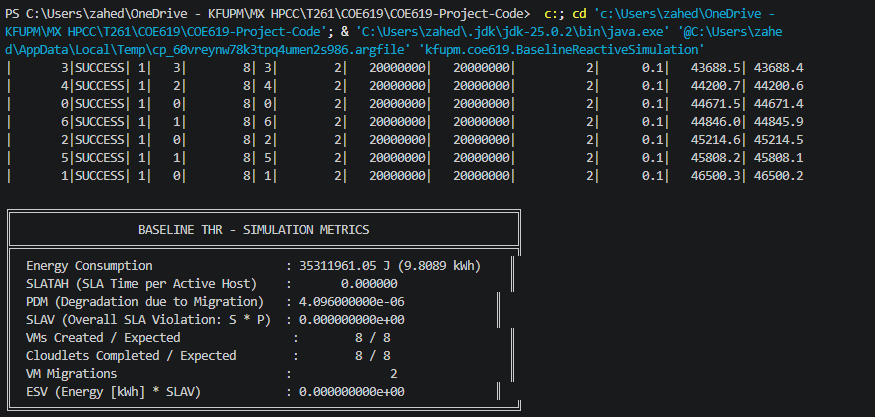
\includegraphics[width=\linewidth]{figures/BaselineReactiveSimulation.png}
\caption{Console output of \texttt{BaselineReactiveSimulation} (THR baseline).}
\label{fig:thr}
\end{figure}

\begin{figure}[H]
\centering
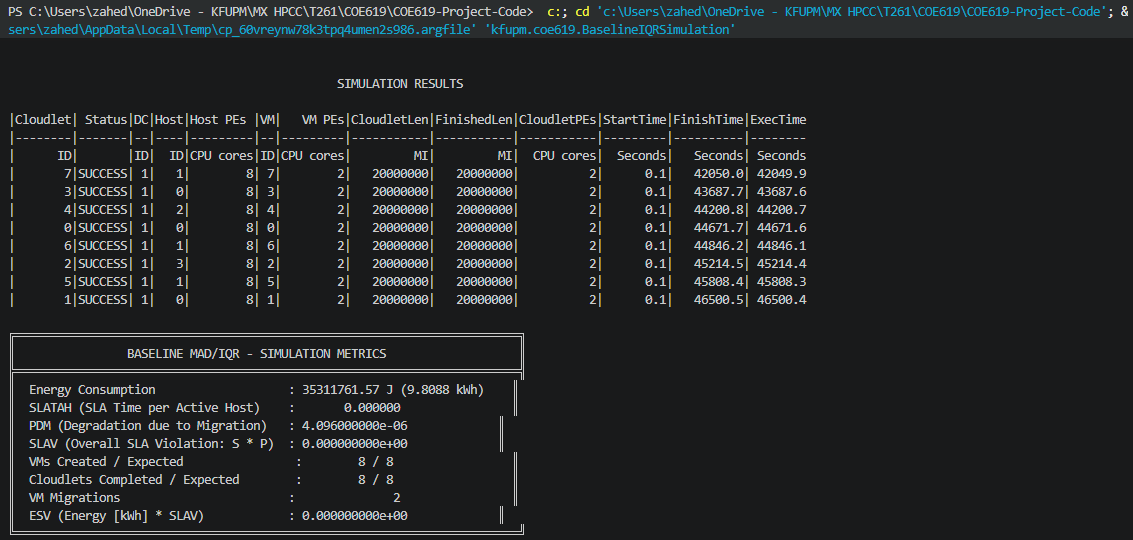
\includegraphics[width=\linewidth]{figures/BaselineIQRSimulation.png}
\caption{Console output of \texttt{BaselineIQRSimulation} (IQR baseline).}
\label{fig:iqr}
\end{figure}

\paragraph{Discussion.} Both policies produced similar results under this synthetic diurnal workload. Their energy differs by approximately 199.48~J (0.000565\%), and their migration counts are equal. Broader experiments are needed; this single run per policy does not establish superiority. No host reached saturation, so SLATAH, SLAV, and ESV are zero. PDM is positive because two migrations occurred.

\section{Limitations}
\begin{itemize}[nosep]
  \item Synthetic traces, a small topology, and one run per policy mean no statistical or generalizable claims can be made yet.
  \item Energy covers the sampled workload window only (excluding the initial interval and the idle tail).
  \item SLATAH uses $u \ge 0.999$ as the saturation condition; this indicates no remaining CPU headroom and does not alone prove unmet demand. PDM relies on an assumed 10\% migration penalty and uses completed requested cloudlet work as an approximation for its requested-work denominator.
  \item SLAV and ESV are composite research metrics~\cite{beloglazov2012ccpe}, not contractual SLA measures.
\end{itemize}

\section{Progress Against Plan and Next Steps}
\begin{table}[H]
\centering
\begin{tabular}{@{}lll@{}}
\toprule
Task (proposal plan) & Planned & Status \\ \midrule
Literature review and environment setup & Week 6 & Done \\
Run baseline reactive algorithms and extract metrics & Week 9 & Done (preliminary) \\
Progress Report I & Week 10 & This report \\
Design predictive model & Week 13 & Next \\
Progress Report II & Week 15 & Planned \\
\bottomrule
\end{tabular}
\caption{Progress against the proposal's time plan (Term 261).}
\end{table}

\noindent Next steps:
\begin{enumerate}[nosep]
  \item Run repeated experiments to quantify variation and evaluate saturation and unmet CPU demand.
  \item Switch to real PlanetLab traces~\cite{park2006comon} and a larger topology. Run repeated experiments and report means and spread.
  \item Design a lightweight predictive overload detector (e.g., linear regression or exponential smoothing on recent host utilization) for Progress Report II.
  \item Implement and compare it against THR and IQR in Term 262, without assuming in advance that it will improve on them.
\end{enumerate}

\begin{thebibliography}{9}
\bibitem{beloglazov2012ccpe}
A.~Beloglazov and R.~Buyya, ``Optimal online deterministic algorithms and adaptive heuristics for energy and performance efficient dynamic consolidation of virtual machines in cloud data centers,'' \emph{Concurrency and Computation: Practice and Experience}, vol.~24, no.~13, pp.~1397--1420, 2012, doi:10.1002/cpe.1867.

\bibitem{cloudsimplus}
M.~C.~Silva~Filho, R.~L.~Oliveira, C.~C.~Monteiro, P.~R.~M.~In\'acio, and M.~M.~Freire, ``CloudSim Plus: A cloud computing simulation framework pursuing software engineering principles for improved modularity, extensibility and correctness,'' in \emph{Proc. IFIP/IEEE Int. Symp. Integrated Network Management (IM)}, 2017, pp.~400--406.

\bibitem{calheiros2011}
R.~N.~Calheiros, R.~Ranjan, A.~Beloglazov, C.~A.~F.~De~Rose, and R.~Buyya, ``CloudSim: A toolkit for modeling and simulation of cloud computing environments and evaluation of resource provisioning algorithms,'' \emph{Software: Practice and Experience}, vol.~41, no.~1, pp.~23--50, 2011.

\bibitem{clark2005}
C.~Clark, K.~Fraser, S.~Hand, J.~G.~Hansen, E.~Jul, C.~Limpach, I.~Pratt, and A.~Warfield, ``Live migration of virtual machines,'' in \emph{Proc. 2nd USENIX Symp. Networked Systems Design and Implementation (NSDI)}, 2005, pp.~273--286.

\bibitem{voorsluys2009}
W.~Voorsluys, J.~Broberg, S.~Venugopal, and R.~Buyya, ``Cost of virtual machine live migration in clouds: A performance evaluation,'' in \emph{Proc. 1st Int. Conf. Cloud Computing (CloudCom)}, LNCS 5931, Springer, 2009, pp.~254--265.

\bibitem{park2006comon}
K.~Park and V.~S.~Pai, ``CoMon: A mostly-scalable monitoring system for PlanetLab,'' \emph{ACM SIGOPS Operating Systems Review}, vol.~40, no.~1, pp.~65--74, 2006.

\bibitem{marinescu2023}
D.~C.~Marinescu, \emph{Cloud Computing: Theory and Practice}, 3rd~ed. Morgan Kaufmann, 2023. (Advisor-recommended; cited for general virtualization concepts.)
\end{thebibliography}

\end{document}
